\documentclass[11pt]{article}
\usepackage[margin=1in]{geometry}
\usepackage{graphicx,booktabs,amsmath,float,caption,subcaption,xcolor,hyperref}
\captionsetup{font=small}
\setlength{\parskip}{4pt}\setlength{\parindent}{0pt}
\newcommand{\fillin}[1]{\textcolor{red}{\textbf{[#1]}}}

\title{HW3: 3D Reconstruction from Images\\\large EE 381V --- Advanced Topics in Computer Vision, Fall 2026}
\author{Yiming Xiong}
\date{}

\begin{document}
\maketitle

All numbers come from the executed notebook, run on a Colab Tesla T4 GPU (PyTorch 2.14, CUDA 13).
The dataset has 160 public and 32 private entries. Among the public entries, 48 training cars have 128 posed views, 32 have 32 posed + 96 unposed, 16 have 16 posed + 112 unposed, 16 have 8 posed, and 16 have 128 unposed. The 32 public test entries are split into 16 with 128 posed views, 8 with 8 posed views and 8 with 1 unposed view (the private set has the same split).

%==================================================================
\section*{Q1: Cameras and rays}

\begin{figure}[H]
\centering
\begin{subfigure}{0.32\textwidth}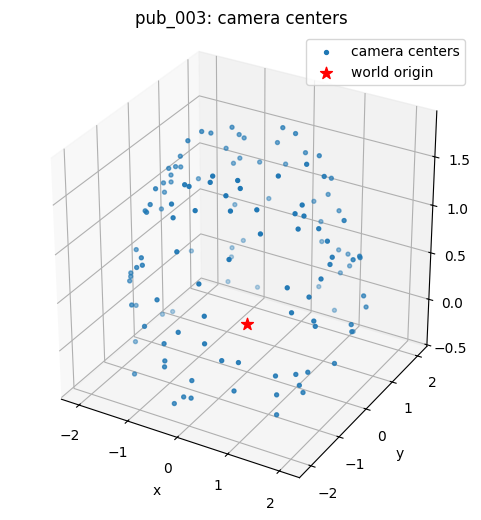
\includegraphics[width=\textwidth]{figs/cam_centers.png}\caption{Camera centers}\end{subfigure}
\begin{subfigure}{0.32\textwidth}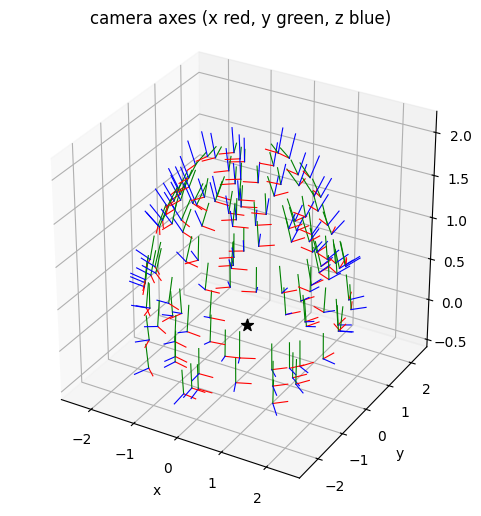
\includegraphics[width=\textwidth]{figs/cam_axes.png}\caption{Camera axes (x red, y green, z blue)}\end{subfigure}
\begin{subfigure}{0.32\textwidth}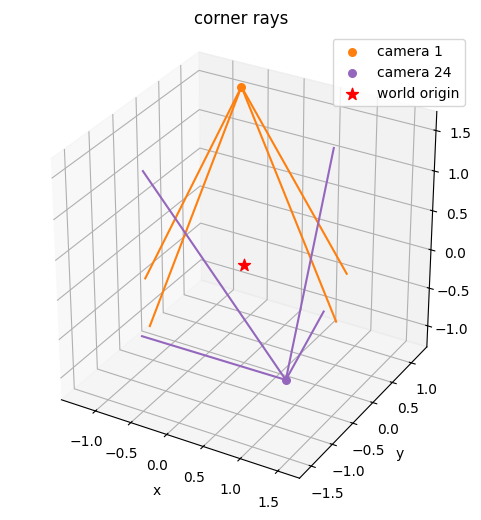
\includegraphics[width=\textwidth]{figs/corner_rays.png}\caption{Corner rays of cameras 1 and 24}\end{subfigure}
\caption{Cameras of \texttt{pub\_003} (128 training views); the star is the world origin.}
\end{figure}

\textbf{Where are the cameras, and where do they look?}
The 128 camera centers lie on a sphere around the origin. Computed over the training cars, the radius is $2.100\pm0.000$, i.e.\ the same for every camera, and the elevation spans $-10^\circ$ to $60^\circ$, so the cameras cover mostly the upper part of the sphere, with a few slightly below the horizon. The world $+z$ axis is ``up'' (the mean camera $y$ axis is $(-0.002, 0.006, 1.0)$). In Fig.\,1b the blue $z$ axes point \emph{away} from the origin. Since a camera looks down its $-z$ axis, every camera looks toward the origin. The green $y$ axes point roughly upward (world $+z$), and the red $x$ axes are horizontal and tangent to the sphere. Thus there is no roll: all cameras are ``look-at'' cameras with the same up vector.

\textbf{Where do the corner rays pass?}
The four corner rays of a camera form a pyramid whose apex is the camera center, and the origin lies inside it, near its axis (Fig.\,1c). At the depth of the origin (2.1) the pyramid cross-section is only about two units wide, so it is only a bit larger than the car, whose visual hull has a half-size of about 0.84. Hence each image covers the whole car with a small margin, and nothing outside the neighborhood of the origin. This is why the white background carries no information, and why a bounding box around the origin is enough as the scene volume.

%==================================================================
\section*{Q2: Single-scene reconstruction (Task 1)}

\textbf{Method.}
I use an explicit voxel grid radiance field (in the style of DVGO / Plenoxels), written in plain PyTorch. A $128^3$ density grid and a $128^3$ grid of 12-channel features are queried by trilinear interpolation. A small MLP (2 hidden layers of 64) maps the interpolated feature and the positionally encoded view direction to RGB. A pixel is rendered by classical volume rendering with 160 samples per ray, and the white background is added to the remaining transmittance. Before training, a coarse visual hull from the white-background silhouettes gives a tight cube around the car, and each ray is only sampled inside this cube. Training uses Adam, 5000 iterations, 4096 rays per step, exponential learning-rate decay ($0.05\to0.005$ for the grids), the photometric MSE loss and a small total-variation penalty on the density grid.

\textbf{Why this representation, and what I rejected.}
A voxel grid has no large network, so each iteration costs only a few lookups, and it needs no extra libraries. I rejected (i) the original NeRF, because it needs hundreds of thousands of large-MLP evaluations per step and is slow on a T4; (ii) 3D Gaussian Splatting, because it needs a custom CUDA rasterizer and a point-cloud initialization (normally from SfM) which is a poor fit for 64$\times$64 images and unreliable with few views; and (iii) a hash-grid (Instant-NGP), because it needs a compiled extension that may not install on Colab.

\textbf{Results} (data entry \texttt{pub\_003}, 128 posed training views, 32 test views):

\begin{center}
\begin{tabular}{lr}
\toprule
Test PSNR (mean of 32 views) & 28.65 dB\\
Final training PSNR & 42.32 dB\\
Reconstruction time (5000 iterations) & 304.6 s\\
Rendering time & 0.63 s for 32 views = 19.8 ms/view\\
Hardware & Tesla T4 (Colab)\\
\bottomrule
\end{tabular}
\end{center}

The 14 dB gap between training and test PSNR shows that the representation fits the training images much more tightly than it generalizes. Training is slower than I would like (about 5 minutes) because of the dense $128^3\times 13$ grid and 160 samples per ray, while rendering is fast since no network has to be queried for empty space.

\begin{figure}[H]
\centering
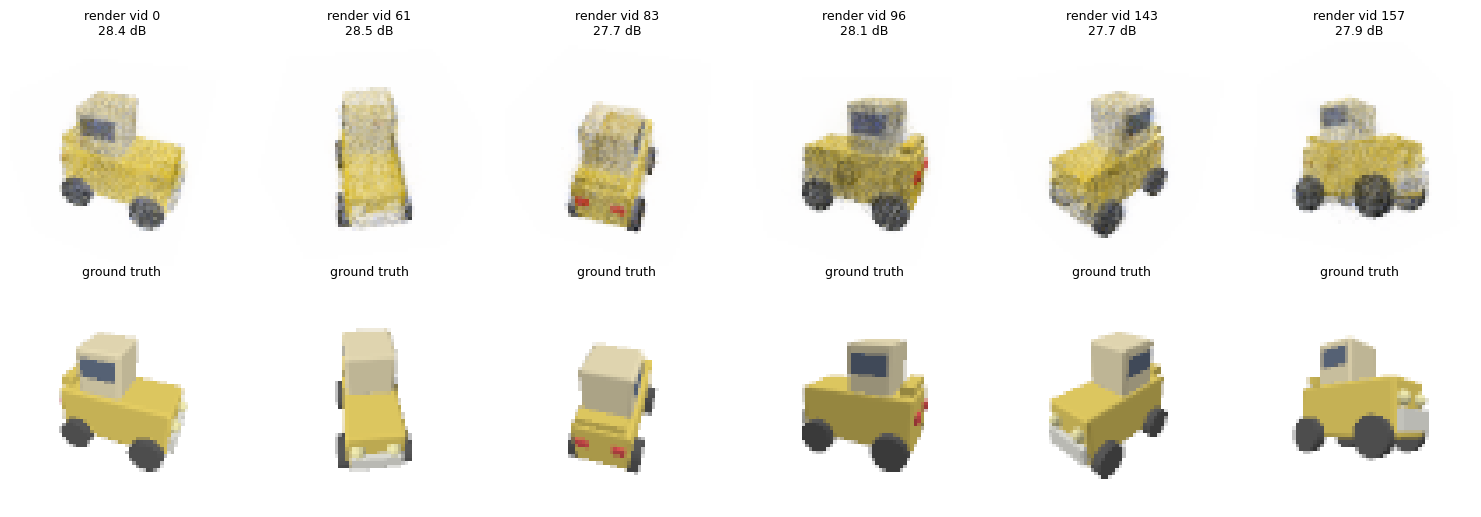
\includegraphics[width=\textwidth]{figs/task1_renders.png}
\caption{Task 1 on \texttt{pub\_003}: renders (top) and ground-truth test images (bottom).}
\end{figure}

\textbf{What works and what does not.}
The overall shape, the wheel positions, the colors and the window are recovered correctly from every viewpoint, and the new views are geometrically consistent. What fails is surface quality: flat-colored faces (roof, hood, side) that are perfectly uniform in the ground truth appear speckled and noisy, the silhouettes are slightly fuzzy with semi-transparent haze at the edges, and thin or low-contrast details (bumper, headlights, tail lights) are blurred. These artifacts are consistent with the PSNR of 28 dB: with 128 views of only $64\times64$ pixels, each voxel is constrained by few rays, and the independent per-voxel parameters absorb noise instead of making a clean surface.

%==================================================================
\section*{Q3: Task 1 method with few views}

The Task 1 method was run unchanged, with a lighter configuration (2000 instead of 5000 iterations). \texttt{pub\_128} has no posed training view, so I assigned its single image a guessed pose: a camera on the $+z$ axis at distance 2.1 looking at the origin.

\begin{center}
\begin{tabular}{lrrr}
\toprule
Case & Train views & Test PSNR (dB) & Recon.\ time (s)\\
\midrule
\texttt{pub\_003}, all views & 128 posed & 28.65 & 304.6\\
\texttt{pub\_003}, subset & 8 posed & 20.03 & 121.8\\
\texttt{pub\_137} & 8 posed & 20.44 & 137.5\\
\texttt{pub\_128} & 1 unposed (guessed pose) & 13.69 & 189.9\\
\bottomrule
\end{tabular}
\end{center}
Rendering time is 0.63--0.66 s per 32 views in all cases.

\begin{figure}[H]
\centering
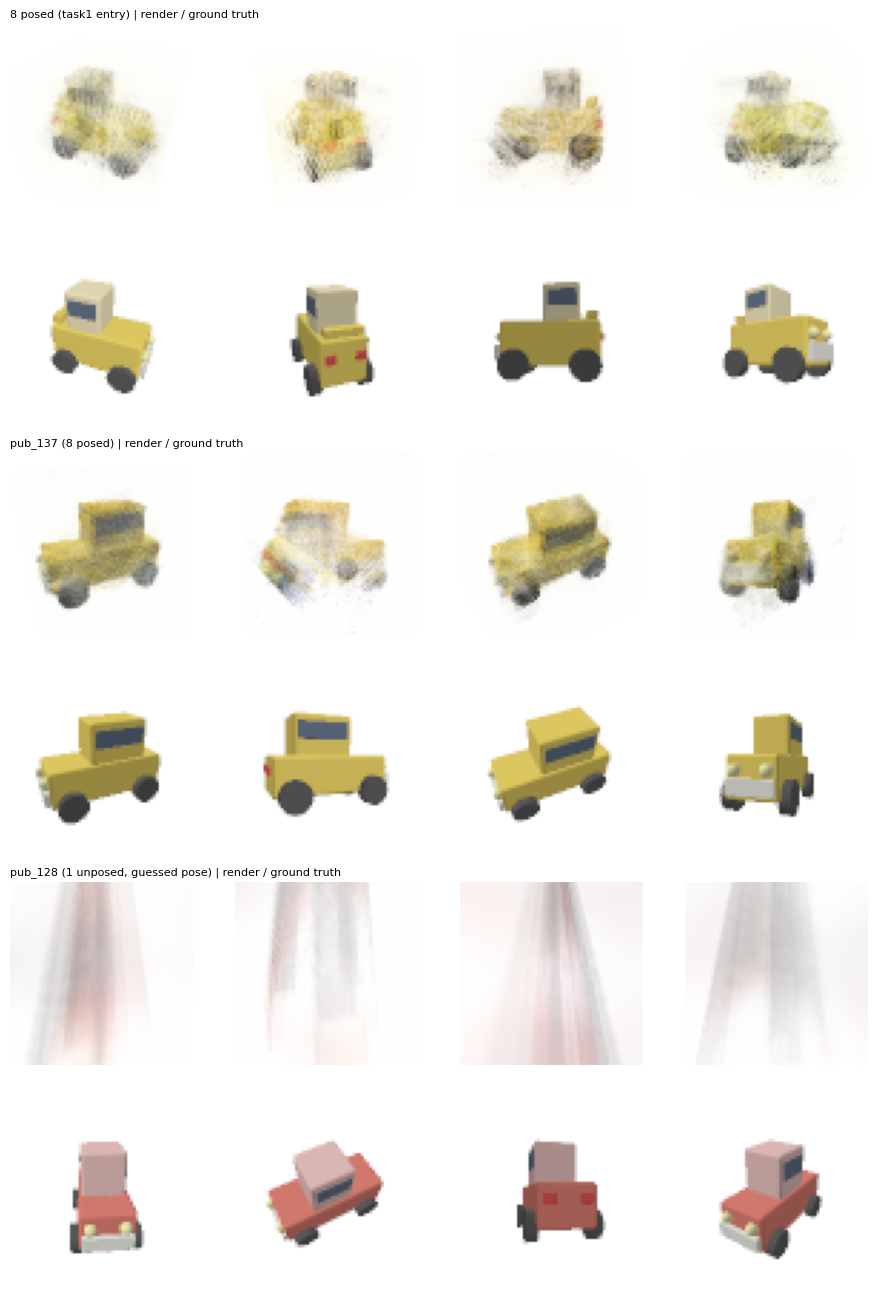
\includegraphics[width=0.62\textwidth]{figs/q3_renders.png}
\caption{Task 1 method on the three harder cases (renders above, ground truth below, four test views each).}
\end{figure}

\textbf{What goes wrong with 8 views.}
The training PSNR is still high (39--46 dB), but the test PSNR drops by about 8 dB. Eight views do not constrain the volume: the grid memorizes the 8 images by putting color wherever it reduces their loss, which produces semi-transparent ``floaters'' and fog in front of and around the car, and streaky artifacts that are only correct from the training directions. Parts of the car that none of the 8 cameras sees (e.g.\ the back or the other side) are never supervised, so they come out as noise or empty space. In \texttt{pub\_137} there are also bluish smudges around the car.

\textbf{What goes wrong with one unposed image.}
The model reaches 48.7 dB training PSNR, so it reproduces the single image perfectly, but the test PSNR is only 13.7 dB, and the renders contain no car at all, only blurry gray--pink streaks. With one image, nothing tells the optimizer where along each ray the color should be, so it spreads it over the whole ray (the depth ambiguity), which gives a fan of streaks from the guessed camera instead of a solid object. On top of that, the guessed pose may be wrong, so even a correct reconstruction would be rendered from the wrong place. The method has no notion of what a car looks like, which is exactly what the prior in the next part adds.

%==================================================================
\section*{Q4: Few-view reconstruction (Task 2)}

\textbf{Approach and the data it uses.}
The key idea is to learn a prior over cars from the other entries of the dataset, as the hint suggests. I train an \emph{auto-decoder}: every training car $i$ gets a latent code $z_i\in\mathbb{R}^{128}$, and one shared decoder (a linear layer followed by four 3D transposed convolutions) maps $z_i$ to a $64^3$ grid with one density channel and 16 feature channels, which a shared MLP and the same volume renderer as in Task 1 turn into images. The codes, the decoder and the MLP are trained jointly with the photometric loss on the posed training views of the 80 public training cars that have at least 32 posed views (48 with 128 posed and 32 with 32 posed views), for 6000 iterations (4 cars $\times$ 1024 rays per iteration). The final training PSNR is 31.7 dB. The cube size and the camera statistics (up direction, radius, elevation range) are also taken from these cars. This is done once, and the prior is stored on disk. The entries with fewer posed views or only unposed views were not used.

For a new car, the decoder stays fixed, and only the 128-dimensional code is optimized (300 Adam steps, started from the mean code, with a small penalty toward it) to fit all the posed training views. This is hard to overfit with 8 images because the search space is tiny and every code decodes to a plausible car.

For unposed images, the camera is parameterized by azimuth, elevation and radius, using the fact (verified in Q1) that all cameras look at the origin with the same up axis. I first score 144 poses (36 azimuths $\times$ 4 elevations) against the image using the mean car, keep the three best, and from each of them jointly refine the code and the pose by gradient descent. The run with the lowest final loss is kept. The three restarts address the front/back ambiguity of a car's silhouette.

\textbf{Results on the public test entries.}

\begin{center}
\begin{tabular}{lrrrr}
\toprule
Kind of entry & $n$ & Task 1 method (PSNR) & Task 2 method (PSNR) & Time / entry\\
\midrule
128 posed & 16 & 28.65 (\texttt{pub\_003}) & 29.65 & 5.5 s\\
8 posed & 8 & 20.03 / 20.44 & 29.93 & 5.5 s\\
1 unposed & 8 & 13.69 (\texttt{pub\_128}) & 23.70 & 19.9 s\\
\midrule
all & 32 & -- & 28.23 & 9.1 s\\
\bottomrule
\end{tabular}
\end{center}

The time is reconstruction plus rendering of 32 views per entry. The prior itself needs to be trained once (\fillin{fill in: training time of the prior on the T4}) and then costs nothing per entry. On the private set, the submission cell reports an average of 8.8 s per entry. The Task 1 numbers come from the single entries of Q2/Q3 (the 8-posed row gives the two entries of Q3), so they are a reference, not a mean over the same entries.

\textbf{Comparison with Task 1.}
With 8 posed views, the prior raises the PSNR from about 20 dB to 29.9 dB (almost +10 dB), and with a single unposed image from 13.7 dB to 23.7 dB (+10 dB), which now gives a recognizable car instead of streaks. The new method is also 10--55 times faster (5.5--19.9 s against 122--305 s). With 128 posed views, the two methods are close (29.65 vs.\ 28.65 dB, on different entries). Note that the Task 2 numbers for 128 posed and 8 posed views are almost identical: the quality is limited by what the decoder can represent (31.7 dB even on its own training cars), not by the number of input views. The 128-view case is therefore the one where per-scene optimization has potential left, for example by starting from the decoded grid and fine-tuning it.

\textbf{Where it still fails.}
\begin{figure}[H]
\centering
\IfFileExists{figs/q4_failures.png}{\includegraphics[width=\textwidth]{figs/q4_failures.png}}{\fbox{\parbox{0.9\textwidth}{\centering\vspace{1.5cm}\fillin{insert figs/q4\_failures.png: renders vs.\ ground truth for the worst cases}\vspace{1.5cm}}}}
\caption{Worst cases of the Task 2 method (renders above, ground truth below).}
\end{figure}
The largest remaining gap is the one-unposed-image case (23.7 dB against about 30 dB with posed views). Likely causes (to be checked against the figure) are: the pose estimate can be wrong, either by the front/back flip or by a few degrees, which moves the whole car in every rendered view, and a single image cannot show the colors of the unseen sides, so they come from the prior and may differ from the truth (e.g.\ the tail lights, or the shade of the opposite side). In all cases, the decoder produces a smoothed car: the fine details (small lights, bumpers) are blurred, because one 128-dimensional code on a $64^3$ grid cannot represent everything. Cars that are unlike the 80 training cars are probably fitted worse, since the prior can only express what it has seen.

\end{document}
